% \begin{center}
%     \captionof{figure}{Bias for DGM 2 in Within-Person and Contextual Effect for Different Estimation Approaches}
%     \begin{subfigure}{1.1\linewidth}
%         \centering
%         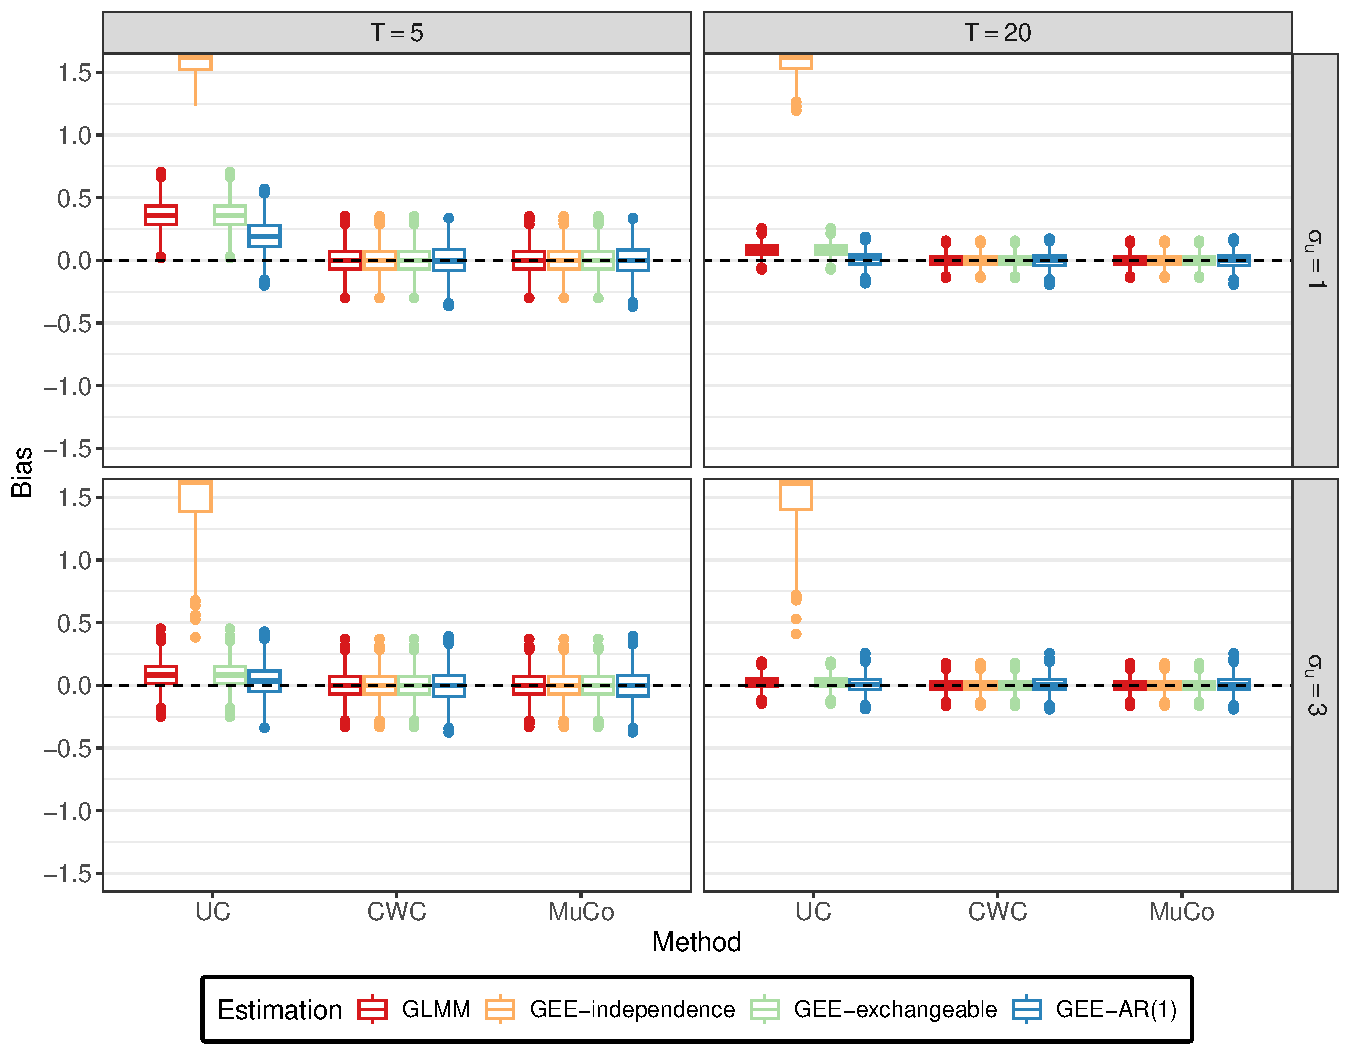
\includegraphics[width=\linewidth, keepaspectratio]{Figures/pred_binary_out_continuous_bias_plot_T_total-vs-sd.u0_within.pdf}
%         \caption{Within-Person Effect}\label{fig:dgm2-within}
%     \end{subfigure}
%     % \hfill
%     \begin{subfigure}{1.1\linewidth}
%         \centering
%         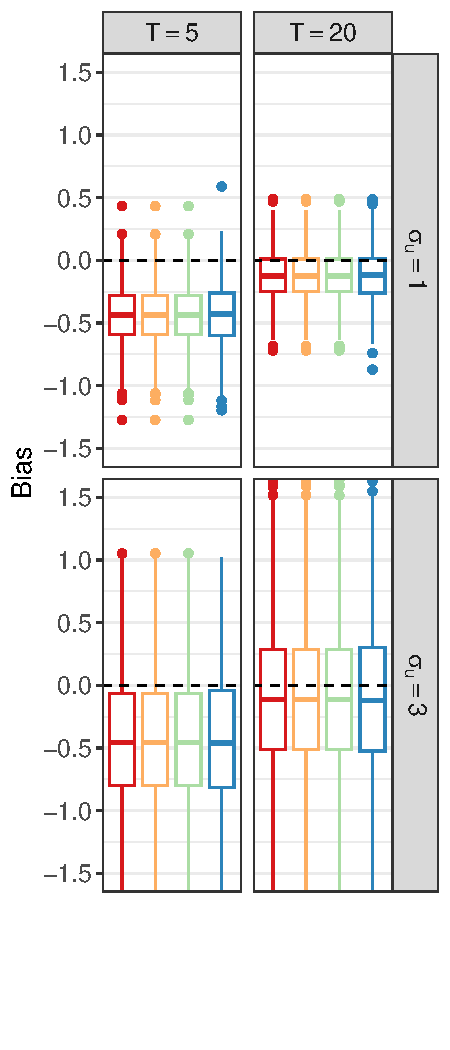
\includegraphics[width=\linewidth, keepaspectratio]{Figures/pred_binary_out_continuous_bias_plot_T_total-vs-sd.u0_contextual.pdf}
%         \caption{Contextual Effect (Method 3)}\label{fig:dgm2-contextual}
%     \end{subfigure}
%     \label{fig:dgm2}
%     % \begin{figurenote}
%     %     \ldots
%     % \end{figurenote}
% \end{center}


\begin{center}
    \captionof{figure}{Bias for DGM 2 in Within-Person and Contextual Effect for Different Estimation Approaches}
     \hspace*{-1.5cm}
    \begin{subfigure}{0.80\linewidth}  % Set width proportionally for the first figure
        \centering
        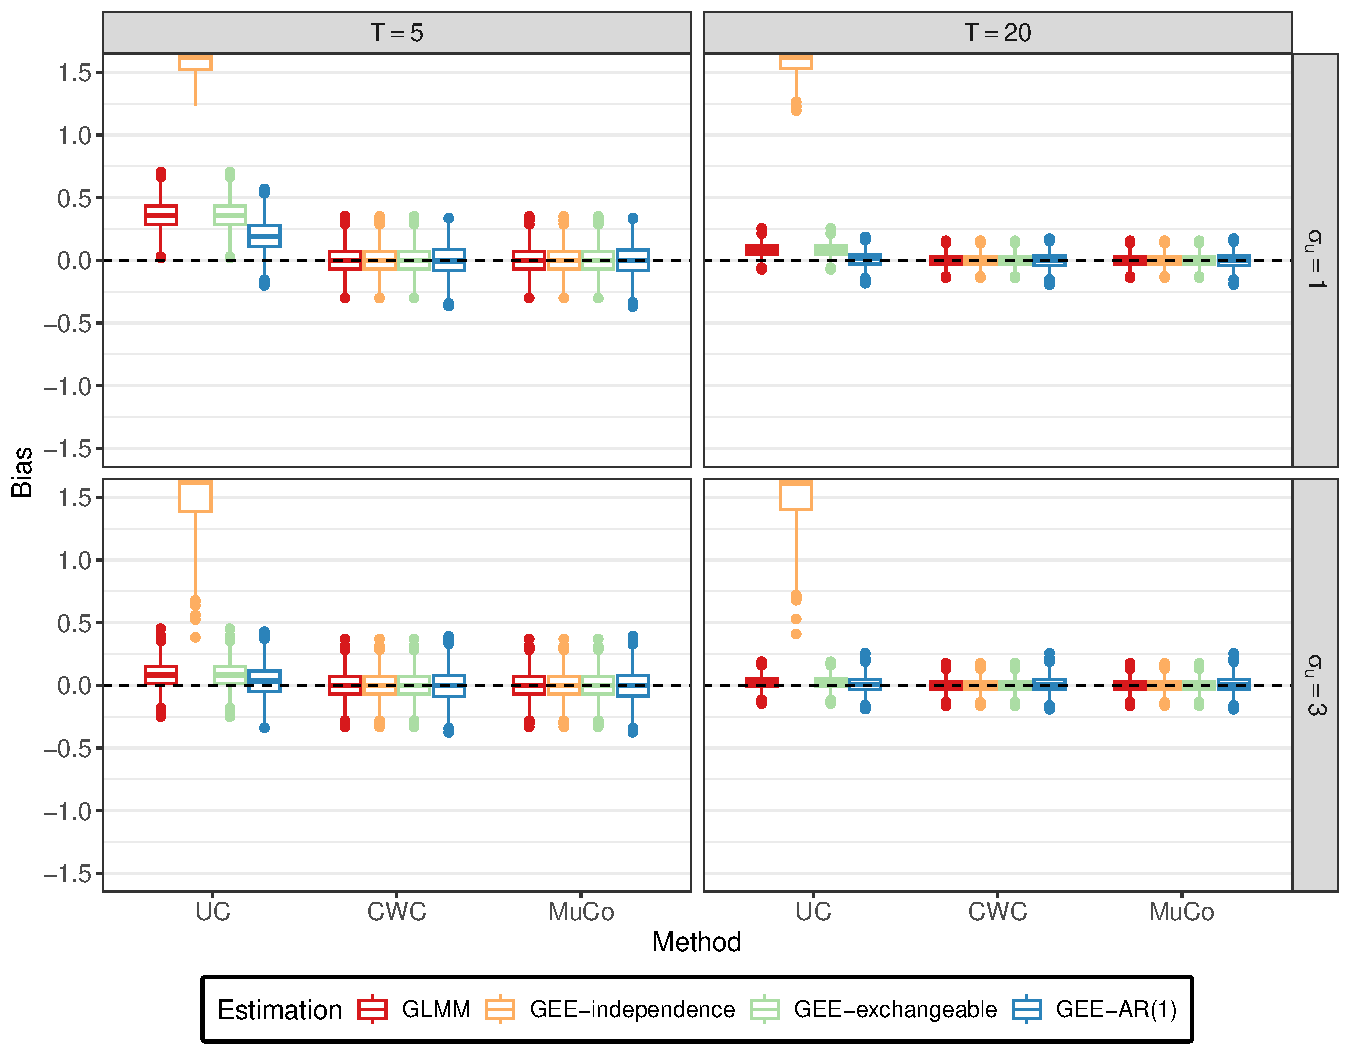
\includegraphics[height=10.6cm, keepaspectratio]{Figures/pred_binary_out_continuous_bias_plot_T_total-vs-sd.u0_within.pdf}
        \caption{Within-Person Effect $\beta_1$}\label{fig:dgm2-within}
    \end{subfigure}
    \hfill
    \begin{subfigure}{0.25\linewidth}  % Set width proportionally for the second figure
        \centering
        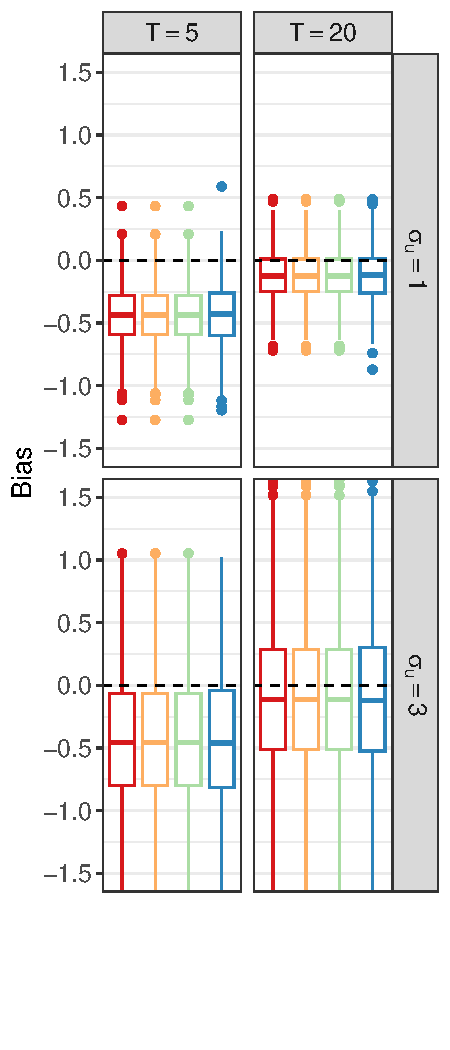
\includegraphics[height=10.6cm, keepaspectratio]{Figures/pred_binary_out_continuous_bias_plot_T_total-vs-sd.u0_contextual.pdf}
        \caption{Contextual Effect $\gamma_{01}$ (Method MuCo)}\label{fig:dgm2-contextual}
    \end{subfigure}
    \label{fig:dgm2}
    \begin{flushleft}
        \begin{figurenote}
        The boxplot shows bias based on 1000 replications for data-generating model 2, which includes a binary predictor and continuous outcome. The boxes represent the interquartile range (IQR) from the 25th to 75th percentiles, with the median indicated by the horizontal line inside. Whiskers extend to 1.5 times the IQR, and replications outside this range are plotted as dots. UC = uncentered, CWC = centered within clusters, MuCo = Mundlak contextual, GLMM = generalized linear mixed model, GEE = generalized estimating equations. $T$ represents the total number of time points, and $\sigma_u$ denotes the random intercept residual variance.

        
        % The boxplot shows bias based on 1000 replications for data-generating model 2, which includes a binary predictor and continuous outcome. The boxes represent the interquartile range from the 25th to 75th percentiles, with the median indicated by the horizontal line inside. Whiskers extend to 1.5 times the IQR, and points outside this range are considered outliers, plotted as dots. UC refers to uncentered, CWC to centered within clusters, and MuCo to Mundlak contextual. $T$ represents the total number of time points, and $\sigma_u$ denotes the random intercept residual variance.
        % Bias is shown for data-generating model 2, which includes a binary predictor and continuous outcome. UC refers to uncentered, CWC to centered within clusters, and MuCo to Mundlak contextual. $T$ represents the total number of time points, and $\sigma_u$ denotes the random intercept residual variance.
    \end{figurenote}
    \end{flushleft}
\end{center}